\documentclass{article}
\usepackage{verbatim}
\usepackage{graphicx}
\usepackage{wrapfig}
\title{\verbatiminput{title.txt} \small{\verbatiminput{version.txt}}}
\author{\input{authors.txt}}
\date{\verbatiminput{date.txt}}
\begin{document}
	\maketitle
	\begin{abstract}
		
	\end{abstract}

\section{Introduction}
EnrichedChem Plugin for Cytoscape is a chemical tool for visualizing compound
similarity in the Cytoscape environment. It supports results from different data
processing programs like Hierarchical Clustering, CMAP and etc. It can search
matched compound from PubChem based on compound name; calculate compound
similarity; connect all compounds according to their similarities and show out
by a network. It provides an easy to use one-key compound search function
searches compound information from Pubchem. The plugin can also be connected to
a Mongo DB database as stream to accelerate all processes.

Compared to a plugin in Cytoscape app market named ChemViz with similar
functions, EnrichedChem has a better function in searching matched compounds
through name, and provides some features ChemViz doesn't have. EnrichedChem also
supports using them together to get more powerful results.

\section{Instruction}

\subsection{Control Panel}
\begin{figure}[ht!]
	\centering
	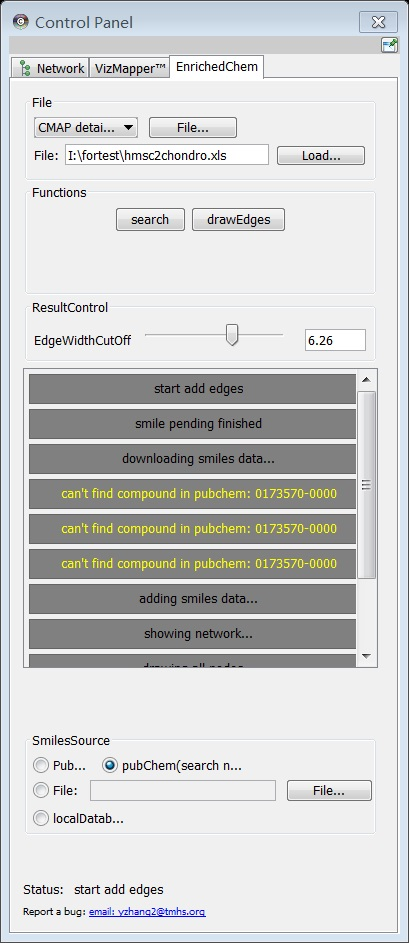
\includegraphics[width=0.4\textwidth]{controlPanel.jpg}
	\caption{controlPanel}
	\label{controlPanel}
\end{figure}
As Figure \ref{controlPanel} shows, the main panel contains a few buttons. 

One is load button with which you can load data from certain files. Another is
search button which helps you search compounds from Pubchem. And a
"drawEdges" button which calculates compound similarity and organizes all nodes
to a network.

You can simply change the edge-width-cut-off value with a slider. The two
compounds whose similarity is smaller than the value will not be connected. The
nodes on the network are organized by their links.

There is a scroll view shows all the information during process. Yellow texts
mean warning and red means error.

\subsection{Load File}
EnrichedChem only supports CMAP detailed result file right now. Click File to
browse to the file and click load to load the file.

\subsection{Search Function}
After CMAP detailed results are loaded. Click this button to search for matched
compounds from PubChem library. Be sure to have an Internet access, or the
plugin won’t work. One thing you should remember is that the plugin only
searches for the compounds you selected. If you want to search all the
compounds, you should leave nothing selected. The search results will be shown
on the search result panel which is on the bottom of the screen (Figure
\ref{searchPanel}).

\begin{figure}[ht!]
	\centering
	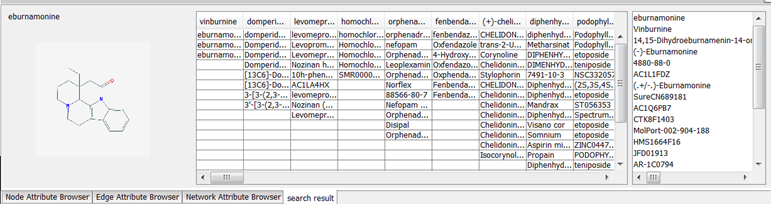
\includegraphics[width=1\textwidth]{searchResults.png}
	\caption{search results panel}
	\label{searchPanel}
\end{figure}

In the middle of the search result panel, all compounds are listed. Every name
has some possible matched compound listed below. Every cell on the table is a
compound. Click on the cell will show the compound’s structure and name on left
and its possible names (alias) on right. We select the first, at the top of the
table, as the default best match. If you want other possible result to be the
best match, just double click on the table cell. The compound will be up to
first and the node’s attributes will be changed.
 
If some compound on the table don’t have results or none of the results matched
well. You can try to modify the name of the compound on the Node Attribute
Brower panel. And select the changed node click search again. The system will
just search for compounds you selected.

\subsection{Draw Edges Function}
If you are satisfied with all the results, you can continue with the draw edge
process. All you need to do is clicking the Draw Edges button.

\subsection{Edge Width Cut Off}


\section{The Network}
The network contains a few graphic elements to indicate different values. For
different file types, the definition is various. Please refer to certain file
instructions below.

But for all file types, the edges’ widths indicate the similarity between the
compounds.

\subsection{CMAP Detailed Results$^{Figure \ref{network}}$}
Here is the define of the graph elements.

Node’s size: the absolute value of score. If the size is bigger, the compound will be more effective.

Color: Red indicates negative value and green indicates positive value.

Pie Chart: The Chart has two parts corresponds to the up and down value.

\begin{figure}[ht!]
	\centering
	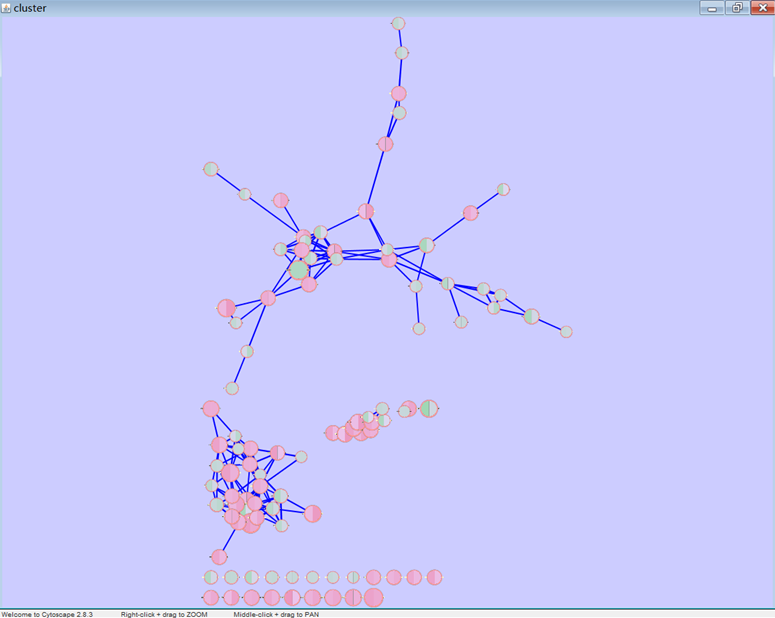
\includegraphics[width=1\textwidth]{network.png}
	\caption{the CMAP network\protect\footnotemark}
	\label{network}
\end{figure}
\footnotetext{This image is from cytoscape 2.x, needs to be updated.}

\section{Release Updates}

\subsection{Version - 2.3.2}
This is a version that sloved all little bugs. But now I don't know what's next.
I also doubt whether this plugin is useful to biologists or chemists. I don't
know what function should be added to it either.

\subsection{Version - 2.3.x}
Version 2.3.0 is a first usable version for cytoscape 3.x. Some bugs may apply
to this version. Like:
\begin{enumerate}
  \item When select nodes, the selected node can't be highlighted.
\end{enumerate}
This version can be release soon because there is no crashing bug. And is stable
according to some test. 

\subsection{Version - 1.4-alpha}
1.x version is capable with Cytoscape 2.x. But as for some reason, the
mutithread process sometimes block the whole Cytoscape environment. This version
will not be released until this bug is fixed.

And this version is made a brunch for developing the Cytoscape 2.x version.

\section{Copyright \& Liscense}


\end{document}